\documentclass[11pt]{article}

% "review" produces the anonymous, line-numbered version required by ARR.
\usepackage[review]{acl}

\usepackage{times}
\usepackage{latexsym}
\usepackage[T1]{fontenc}
\usepackage[utf8]{inputenc}
\usepackage{microtype}
\usepackage{graphicx}
\usepackage{amsmath,amssymb,amsthm}
\usepackage{booktabs}
\usepackage{multirow}
\usepackage{pifont}
\usepackage{enumitem}
\usepackage{eso-pic}
\usepackage{tikz}
\usetikzlibrary{positioning,arrows.meta,calc}
\usepackage{pgfplots}
\pgfplotsset{compat=1.17}

% ======================================================================
% PLACEHOLDER MACHINERY
% Every number that must come from an experiment is written as \ph{...}.
% While \placeholderstrue is set, such numbers print in red, each page
% carries a red draft banner, and Appendix A states the draft status.
% Switching to \placeholdersfalse makes any remaining \ph{...} a compile
% ERROR, so the paper cannot be built for submission until every
% placeholder has been replaced by a measured value (typed without \ph).
% ======================================================================
\newif\ifplaceholders
\placeholderstrue
\newcommand{\ph}[1]{%
  \ifplaceholders\textcolor{red}{#1}%
  \else\PackageError{draft}{Placeholder value `#1' has not been replaced}%
       {Replace every \string\ph{...} by a measured number before submission.}%
  \fi}
\newcommand{\phmark}{\ifplaceholders
  \node[red, font=\tiny\bfseries, rotate=14, opacity=0.5]
     at (rel axis cs:0.5,0.5) {PLACEHOLDER DATA};\fi}
\ifplaceholders
\AddToShipoutPictureBG{\AtPageUpperLeft{\raisebox{-0.9cm}{\hspace{2.5cm}%
  \textcolor{red}{\footnotesize\sffamily DRAFT. Every number printed in red is a
  placeholder, not a measurement. Not for submission in this state.}}}}
\fi

% ---------- shorthands ----------
\newcommand{\method}{Ledger-RM}
\newcommand{\cmark}{\ding{51}}
\newcommand{\xmark}{\ding{55}}
\newcommand{\up}{$\uparrow$}
\newcommand{\dn}{$\downarrow$}
\newcommand{\xf}{x^{\mathrm{f}}}
\newcommand{\xn}{x^{\mathrm{n}}}
\newcommand{\xm}{x^{\mathrm{m}}}
\newcommand{\xp}{x^{\mathrm{p}}}
\newcommand{\bb}{Qwen3-8B}
\newtheorem{proposition}{Proposition}
\setlist{nosep,leftmargin=*}

\title{Learning When to Change: Symbolic Supervision for\\
Selective Evidence Sensitivity in Medical Reward Models}

\author{Anonymous ACL submission}

\begin{document}
\maketitle

\begin{abstract}
Reward models decide which medical reasoning traces are kept, reranked and
reinforced. A useful reward reverses its preference when decisive patient
evidence changes and holds it when similar-looking evidence does not apply: a
penicillin allergy in the patient is a reason to change an order, the same
allergy in the patient's mother is not. We test this \emph{selective
sensitivity} with symbolic triplets from executable, stated clinical rules: a
base case, a flip of one decisive input, and a near-miss that mentions the
same concept without making it applicable. Labels are exact relative to the
stated rule. Across \ph{13} reward signals, \ph{14}--\ph{75}\% of triplets are
solved: trained medical PRMs seldom reverse, and general judges reverse on
near-misses. Balanced sampling teaches reversal, flip pairs alone teach
over-triggering, and near-misses remove most of it. A reader that records each
finding with its subject, status and time, followed by a judge with no direct
access to the case, solves \ph{79}\% of triplets on rules of held-out
structure, \ph{12} points more than a free-form evidence summary under the
same two-stage interface. Trained on rules alone, with no medical QA data, the
model raises agreement with MedEinst pair labels from \ph{18}\% to \ph{45}\%.
Outside rules, selectivity is tested only indirectly, since existing clinical
benchmarks contain no case edits of this kind.
\end{abstract}

\section{Introduction}

A reward model for medical reasoning is asked whether a step or an answer is
right for the patient at hand. Often the answer turns on one line of the case.
Under a rule that orders amoxicillin for streptococcal pharyngitis unless the
patient is allergic to penicillin, the order is right for a patient with no
drug allergy and wrong for one with a documented penicillin allergy
(Figure~\ref{fig:example}). It is right again for a patient whose mother has
that allergy. A reward that prefers the same order in all three cases fails to
reverse when required. One that changes its preference in the second and the
third reverses under an edit that leaves the decision unchanged.

\begin{figure}[t]
\centering\footnotesize
\parbox{0.97\linewidth}{%
\textbf{Stated rule.} Strep.\ pharyngitis: order amoxicillin; if the patient is
allergic to penicillin, order azithromycin.\\
\textbf{Claims.} $s$: ``Order amoxicillin.'' \ \ $s'$: ``Order azithromycin.''}
\\[3pt]
\setlength{\tabcolsep}{3pt}
\begin{tabular}{@{}llccc@{}}
\toprule
Case & Reports & Rule & PRM & \method\\
\midrule
base $x$      & allergies: none          & $s$  & \ph{+1.9} & \ph{+4.2}\\
flip $\xf$    & allergy: penicillin      & $s'$ & \ph{+1.7} & \ph{$-$3.9}\\
near $\xn$    & mother: penicillin all.  & $s$  & \ph{+1.8} & \ph{+3.6}\\
missing $\xm$ & allergies not recorded   & --   & \ph{+1.6} & rejects both\\
\bottomrule
\end{tabular}
\caption{One rule, four cases. Numbers are the preference
$d=u(s)-u(s')$. A PRM trained on injected step errors prefers the default
order throughout; \method{} reverses on the flip and holds on the near-miss.}
\label{fig:example}
\end{figure}

Both failures matter because reward models filter training traces
\citep{chen2024huatuo}, rerank candidates \citep{snell2025scaling,yun2025medprm}
and supply the reward in reinforcement learning
\citep{shao2024deepseekmath,guo2025deepseekr1}. The first is documented: LLM
judges are more reliably invariant to irrelevant edits than sensitive to
relevant ones \citep{chen2026judge}, and clinical LLMs mention a changed
patient fact in 85.6\% of their rationales while keeping the original
medication choice in 69.8\% \citep{hou2026medpic}. The second is easy to
overlook: an output change after a targeted edit means little unless it exceeds
the change after an edit that should not matter \citep{yang2026compared}.
Medical reward models are evaluated on answer selection and on injected step
errors \citep{yun2025medprm,wu2026medprmbench}, neither of which changes the
case. Formal supervision transfers to informal tasks \citep{kamoi2026fover};
which interventions teach a reward when evidence applies is open.

We build the test from executable rules (\S\ref{sec:twins}). Each rule yields
\emph{triplets}: a base case, a \emph{flip} of one decisive input, and a
\emph{near-miss} in which the decisive concept appears without counting under
the rule: in a relative, negated, at a time the rule does not count, or as a
value that approaches a threshold without crossing it. Each case is crossed
with the two claims the rule can support, and the rule program labels all six
instances. Labels state what a stated rule implies, not what is clinically
best. Clinical benchmarks with existing labels form a second tier, where each
measures a different construct (Table~\ref{tab:sources}). Our contributions:

\noindent\textbf{(1) A test.} Triplets separate two failures that pair tests
conflate. Across \ph{13} reward signals \ph{13.8}--\ph{75.0}\% of triplets are
solved (\S\ref{sec:results-audit}).

\noindent\textbf{(2) A controlled comparison} of training distributions and
intermediate representations under one interface and budget
(\S\ref{sec:results-factorial}): balance teaches reversal, flip pairs alone
teach over-triggering, near-misses correct it, and a typed applicability
ledger adds \ph{12.1} points over a free-form summary read by the same
case-blind judge. On rules the gain lies in what the reader is trained to
record: a judge given one applicability bit does almost as well.

\noindent\textbf{(3) Transfer with its confounds removed.} A model trained on
rule triplets only reaches \ph{78.6}\% on rules of held-out structure and
raises agreement with MedEinst labels from \ph{18.4}\% to \ph{44.8}\% without
medical QA data (\S\ref{sec:results-shift}).

\begin{figure*}[t]
\centering
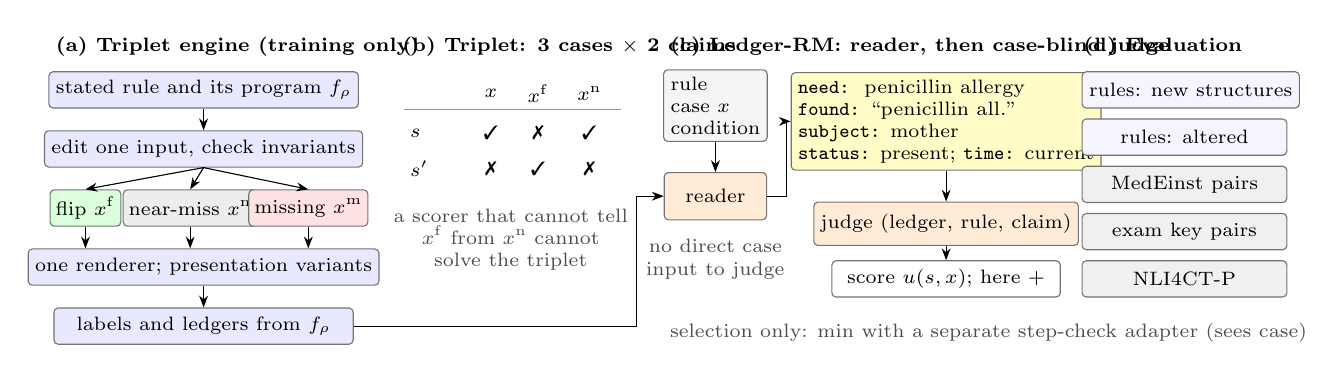
\begin{tikzpicture}[font=\scriptsize, >={Stealth[length=1.5mm]},
  box/.style={draw=black!55, rounded corners=1.5pt, align=center,
              inner sep=2.5pt, minimum height=4.6mm},
  sym/.style={box, fill=blue!9},
  neu/.style={box, fill=orange!16},
  hd/.style={font=\scriptsize\bfseries, anchor=west}]
\node[hd] at (-0.05,3.55) {(a) Triplet engine (training only)};
\node[sym, minimum width=38mm] (rule)   at (1.95,3.0)  {stated rule and its program $f_\rho$};
\node[sym, minimum width=38mm] (search) at (1.95,2.25) {edit one input, check invariants};
\node[box, fill=green!14, minimum width=8mm, inner sep=2pt] (flip) at (0.45,1.5) {flip $\xf$};
\node[box, fill=black!7,  minimum width=13mm, inner sep=2pt] (null) at (1.78,1.5) {near-miss $\xn$};
\node[box, fill=red!11,   minimum width=10mm, inner sep=2pt] (miss) at (3.28,1.5) {missing $\xm$};
\node[sym, minimum width=38mm] (render) at (1.95,0.75) {one renderer; presentation variants};
\node[sym, minimum width=38mm] (check)  at (1.95,0.0)  {labels and ledgers from $f_\rho$};
\draw[->] (rule) -- (search);
\draw[->] (search.south) -- (flip.north);
\draw[->] (search.south) -- (null.north);
\draw[->] (search.south) -- (miss.north);
\draw[->] (flip.south) -- (flip.south |- render.north);
\draw[->] (null.south) -- (null.south |- render.north);
\draw[->] (miss.south) -- (miss.south |- render.north);
\draw[->] (render) -- (check);
\node[hd] at (4.35,3.55) {(b) Triplet: 3 cases $\times$ 2 claims};
\node at (5.6,2.95) {$x$};
\node at (6.2,2.95) {$\xf$};
\node at (6.85,2.95) {$\xn$};
\draw[black!40] (4.5,2.75) -- (7.25,2.75);
\node[anchor=west] at (4.45,2.45) {$s$};  \node at (5.6,2.45) {\cmark}; \node at (6.2,2.45) {\xmark}; \node at (6.85,2.45) {\cmark};
\node[anchor=west] at (4.45,2.00) {$s'$}; \node at (5.6,2.00) {\xmark}; \node at (6.2,2.00) {\cmark}; \node at (6.85,2.00) {\xmark};
\node[text=black!70, align=center] at (5.85,1.1) {a scorer that cannot tell\\ $\xf$ from $\xn$ cannot\\ solve the triplet};
\node[hd] at (7.75,3.55) {(c) \method{}: reader, then case-blind judge};
\node[box, fill=black!4, align=left, minimum width=13mm] (inp) at (8.45,2.8)
     {rule\\ case $x$\\ condition};
\node[neu, minimum width=13mm, minimum height=6mm] (reader) at (8.45,1.65) {reader};
\node[box, fill=yellow!22, align=left, minimum width=29mm] (ledger) at (11.38,2.6)
     {\texttt{need:}\ \ penicillin allergy\\ \texttt{found:} ``penicillin all.''\\
      \texttt{subject:} mother\\ \texttt{status:} present; \texttt{time:} current};
\node[neu, minimum width=29mm, minimum height=5.5mm] (judge) at (11.38,1.3) {judge (ledger, rule, claim)};
\node[box, fill=white, minimum width=29mm] (verdict) at (11.38,0.6) {score $u(s,x)$; here $+$};
\draw[->] (inp) -- (reader);
\draw[->] (reader.east) -- ++(0.25,0) |- (ledger.west);
\draw[->] (ledger) -- (judge);
\draw[->] (judge) -- (verdict);
\node[text=black!70, align=center] at (8.45,0.85) {no direct case\\ input to judge};
\node[text=black!70, anchor=west] at (7.75,-0.08) {selection only: min with a separate step-check adapter (sees case)};
\draw[->] (check.east) -- (7.45,0.0) |- (reader.west);
\node[hd] at (13.0,3.55) {(d) Evaluation};
\node[box, anchor=west, fill=blue!4,   minimum width=26mm] at (13.1,3.0) {rules: new structures};
\node[box, anchor=west, fill=blue!4,   minimum width=26mm] at (13.1,2.4) {rules: altered};
\node[box, anchor=west, fill=black!6,  minimum width=26mm] at (13.1,1.8) {MedEinst pairs};
\node[box, anchor=west, fill=black!6,  minimum width=26mm] at (13.1,1.2) {exam key pairs};
\node[box, anchor=west, fill=black!6,  minimum width=26mm] at (13.1,0.6) {NLI4CT-P};
\end{tikzpicture}
\caption{Overview. The rule program (blue) supervises reader and judge and is
not executed at inference. The reader records findings with subject, status
and time; the judge scores the claim from the ledger and the rule, with no
direct case input. A string check on quotations is the only symbolic operation
at inference.}
\label{fig:overview}
\end{figure*}

\section{Related Work}

\paragraph{Validity of evaluators.}
\citet{chen2026judge} define a judge's validity as invariance to
construct-preserving edits together with sensitivity to construct-changing
ones. \citet{yang2026compared} show that the effect of a targeted
counterfactual edit must be compared with that of meaning-preserving edits of
the same size; our near-miss and presentation edits are such baselines with
known labels. Robustness work on reward models
targets response-side artifacts
\citep{liu2025rrm,srivastava2026crome,zang2025auditor,xu2025contextualjudge}.
The closest is DynaCF, which rewrites the chosen response without changing its
content and down-weights training pairs whose margin shifts or flips
\citep{liu2026dynacf}; its edits should not matter and serve as probes,
whereas we edit the case in both directions and train on the edits, whose
labels are exact. CSR regularises a solver to change its answer when an
operator in its own trace is swapped \citep{shihab2025csr}.

\paragraph{Process rewards and symbolic supervision.}
PRMs are trained on human step labels \citep{lightman2024verify}, rollout
estimates \citep{wang2024mathshepherd} or generated verification reasoning
\citep{khalifa2025thinkprm}, which GenPRM extends with executed code
\citep{zhao2025genprm}. FoVer trains step verifiers on
labels from formal tools and shows transfer to informal tasks including NLI
\citep{kamoi2026fover}, so transfer of formal supervision is not our claim;
we ask which interventions teach applicability and compare with a model
trained on FoVer's data. Other work perturbs steps and keeps a verifier at
inference \citep{zi2026nsprm}, injects errors into verified chains
\citep{chi2026vcs}, or uses a deterministic verifier as the reward
\citep{pronesti2026vprm}. In medicine, Med-PRM verifies steps against
retrieved guidelines \citep{yun2025medprm}, MedCEG rewards a policy for covering
a reference evidence graph built for each training question
\citep{medceg2025}, and MedPRMBench injects 14 error types into
chains from seven QA sources \citep{wu2026medprmbench}. MedGuideX compiles
guideline recommendations into executable functions and post-trains a clinical
policy on factual and counterfactual questions generated from them, keeping
only interventions that change the outcome \citep{shen2026medguidex};
executable guideline functions are also called at inference
\citep{cao2026guideskill}. None of these evaluates a
reward model on a changed case. Mediating a reward through
concepts \citep{koh2020cbm,laguna2025cbrm} precedes our ledger, as does EVPV,
which extracts visual facts once per problem, independently of the solution,
and attenuates the reward of steps whose stated premises they do not support
\citep{evpv2026}. The fields of our ledger are the attributes that clinical
NLP assigns to mentions of findings: negation, experiencer and temporality
\citep{chapman2001negex,harkema2009context,uzuner2011i2b2}. Typed evidence
records and distractors that are similar but irrelevant have been studied in
retrieval \citep{zhou2026fincards,agand2026venra,chen2026deepera}, and
conditional QA asks for answers that change with a stated patient condition
\citep{parekh2026cgr}. The space left open is the reward model: a test with
near-misses whose labels are exact, their use as supervision, and a judge that
sees only the record.

\paragraph{Context against prior, and counterfactual data.}
How language models arbitrate between memory and conflicting context is well
studied \citep{xu2024conflicts,wu2024clasheval,shi2024cad}. Clinical
policies keep the prototypical answer when decisive evidence changes
\citep{chen2026medeinst,hou2026medpic,kim2025marc,qu2026medieval}, and
clinical-trial NLI has been probed with label-preserving and label-inverting
interventions \citep{jullien2024semeval}. Minimal label-flipping edits serve
training \citep{kaushik2020cad} and evaluation
\citep{gardner2020contrast,ribeiro2020checklist,thrush2022winoground}, with
the caveat that narrow edits may not help out of distribution
\citep{joshi2022cad}; claim-only scorers are partial-input baselines
\citep{poliak2018hypothesis}.

\section{Triplets from Two Tiers}
\label{sec:twins}

\subsection{Rule tier}

\paragraph{Rules, states, claims.}
A rule $\rho$ has criteria $c_1,\dots,c_m$ over typed inputs. A patient state
$z$ is a set of \emph{mentions}; each has a concept, a value, a subject
(patient or other), a status (present, absent, unknown) and a time (current or
past). Every criterion $c_j$ comes with an \emph{applicability predicate}
$A_j$ that says which mentions it counts. The predicate is part of the rule:
a creatinine threshold counts the patient's current value, a stroke-risk score
counts a stroke at any time, and some risk scores count disease in a
first-degree relative. In \ph{23}\% of criteria a past or family finding
counts, so no global heuristic about time or subject is correct.
\emph{Scoring rules} are clinical calculators, with claims of the form
``criterion $j$ adds $b$ points''. \emph{Constraint rules} state a decision in
full: choose $a$ unless condition $c$ holds, then $b$; the claims are the two
options in neutral wording of matched length. The prompt states the rule. A
contraindication can exclude an order, and no single rule establishes that an
alternative is optimal; our labels claim only the former kind of fact.

\paragraph{Edits and invariants.}
The engine edits the mentions of one input of a criterion $c_j$ and keeps an
edit only if executing the program confirms its invariant. A \emph{flip}
changes a mention that $A_j$ counts so that $c_j$ changes and no other
criterion does. A \emph{near-miss} leaves every criterion unchanged; it is
\emph{numeric} (a counted value moves toward the threshold without crossing)
or concerns \emph{applicability} (the concept and value of the flip are
reported in a mention that $A_j$ does not count: another subject, absent
status, or a time outside $A_j$). A \emph{presentation} edit re-renders the
same state with another unit, order or template, matched in size to the flips
\citep{yang2026compared}. For \emph{missing} twins we distinguish explicit
absence, which determines a criterion, from an unknown input. Measured inputs
are unknown when omitted; history items are absent when omitted, as in the
source benchmarks, and unknown only when the case says so (``allergies not
recorded''). With $C_\rho(z')$ the completions of a partial state $z'$ within
the input ranges, a missing twin is kept only if
$|\{c_j(z): z\in C_\rho(z')\}|>1$. A verdict ``$+$'' means the claim is
supported by the case under the rule; ``$-$'' covers refuted and undetermined
claims, which verifiers for retrieval keep apart
\citep{qiu2026surerag,kamelhar2026gsar} and we report separately.

\paragraph{Triplets.}
A triplet crosses a base case $x$, its flip $\xf$ and a near-miss $\xn$ with
the claims $s$ (correct for $x$ and $\xn$) and $s'$ (correct for $\xf$). For a
reward with score $u(s,x)$ let $d(x)=u(s,x)-u(s',x)$. The triplet is
\emph{solved} if $d(x)>0$, $d(\xf)<0$ and $d(\xn)>0$; ties are failures.

\begin{proposition}
\label{prop:blind}
Let $u$ be deterministic. (i) If $u(s,x)=g(s)$, then $d(x)=d(\xf)$. (ii) If
$u(s,x)=g(x)$, then $d\equiv 0$. (iii) If $u(s,x)=g(s,h(x))$ for a feature map
$h$ with $h(\xf)=h(\xn)$, then $d(\xf)=d(\xn)$. In each case the triplet is
not solved; under (iii) a correct reversal on the flip implies failure on the
near-miss.
\end{proposition}
\noindent\emph{Proof.} (i) and (ii) are immediate from the definition of $d$.
(iii) $d(\xf)=g(s,h(\xf))-g(s',h(\xf))=g(s,h(\xn))-g(s',h(\xn))=d(\xn)$, while
a solved triplet needs $d(\xf)<0<d(\xn)$. \hfill$\square$

\smallskip
Let $h_k(x)\in\{0,1\}$ indicate whether the decisive concept $k$ is named
anywhere in the case, whatever its value, subject, status or time. For a
finding that the flip introduces, the base case is rendered without naming
$k$ and an applicability near-miss names it, so $h_k(x)=0$ and
$h_k(\xf)=h_k(\xn)=1$: (iii) applies. For a measured input $k$ is named in
all three cases, so $d(x)=d(\xf)$ as in (i). A scorer that uses the case only
through $h_k$ thus solves no triplet, although it can reverse on every flip of
the first kind. Richer attribute-blind features need not collide and are an
empirical baseline (Appendix~\ref{app:diag}). Flip pairs alone exclude only (i) and (ii). With
sampled scores the statement holds in expectation, and finite samples can show
apparent reversals; we report tie rates and sampling intervals.

\paragraph{Metrics.}
\emph{Reversal} (Rev): share of base--flip pairs with $d(x)>0$ and
$d(\xf)<0$. \emph{Hold}: share of near-misses with $d(\xn)>0$. \emph{Triplet
accuracy} (TA): share of solved triplets, the primary summary. None needs a
threshold. Base accuracy, ties, and the conditional rate of unnecessary
reversal with its denominator are in Appendix~\ref{app:diag}. For missing
twins, MR is the rate at which both claims are rejected at the threshold that
gives \ph{5}\% false rejection of supported claims on development data.

\subsection{Clinical tier}

Labels that we generate with one model and approve with another would not be
ground truth, so the clinical tier uses only released labels. Each source
supports a different statement (Table~\ref{tab:sources}).

\begin{table}[t]
\centering\small
\setlength{\tabcolsep}{3pt}
\begin{tabular}{@{}p{1.6cm}p{2.55cm}p{2.95cm}@{}}
\toprule
Source & Label basis & What it can show\\
\midrule
Rule triplets & executed program of a stated rule & reversal and holding under that rule; exact\\
MedEinst & DDXPlus cases, edited and filtered by the benchmark & agreement with labels across paired diagnostic cases\\
Key pairs & answer keys of two exam questions & paired answer discrimination\\
NLI4CT-P & expert labels, controlled interventions & response to statement edits, report fixed\\
\bottomrule
\end{tabular}
\caption{Sources and constructs. Only the first contains near-misses.}
\label{tab:sources}
\end{table}



\emph{MedEinst} \citep{chen2026medeinst} pairs a control case with a trap case
that differs in discriminating findings and has another diagnosis (5,383 test
pairs; 10,689 reference pairs). \emph{Key pairs} are two exam questions whose
keyed answers each occur among the other's options. A claim is the complete
question with one candidate answer, so the four labels follow from the keys.
We exclude negatively phrased questions and options that refer to other
options, and keep each question in at most one pair. Two exam questions are
not a controlled counterfactual; the test measures discrimination between
answers given the case. We mine pairs from MedQA \citep{jin2021medqa} and
CareQA \citep{ariasduart2025careqa}. \emph{NLI4CT-P} \citep{jullien2024semeval}
edits expert-written statements about trial reports; we report its
faithfulness and consistency with base F1.

\section{Diagnostics}
\label{sec:diagnostic}

\paragraph{Parts and whole.}
For each base--flip pair we build a \emph{reading} pair, whose claims quote
the decisive finding, and an \emph{application} pair, which scores the
original claims against a one-line case with only that finding. With $P$, $K$,
$U$ the events of a correct reversal on the three pairs, the composition gap
is $G=1-\Pr[U\mid P\wedge K]$; it is descriptive, since the tasks differ in
length and in what must be selected.

Appendix~\ref{app:diag} analyses how far, and in which direction, a decisive
edit moves the preference relative to a missing-input baseline.

\section{\method}
\label{sec:ledger}

\paragraph{Reader.}
The reader $R_\phi$ receives the case $x$, the rule $\rho$ where one is
stated, and the \emph{condition under test} $\omega$: the criterion, or the
set of candidate answers, on which the claims disagree. It does not receive a
candidate's asserted outcome, so the claims of a triplet are judged from one
ledger $e=R_\phi(x,\rho,\omega)$ of up to \ph{3} entries. An entry records
facts and no decision: the condition the claim depends on
(\texttt{need}); what the case says about it (\texttt{found}: a value with
unit, a verbatim quotation, or \texttt{missing}); whose finding it is
(\texttt{subject}); its \texttt{status} (present, absent, unknown); and its
\texttt{time} (current or past). Keys and categorical fields are fixed by a
grammar, and a quotation that does not occur in the case makes the ledger
malformed.

\paragraph{Judge.}
The judge $J_\phi$ receives the ledger, the rule if any, and the claim, and
decides whether the recorded finding counts under the rule and what follows
for the claim. The end-to-end score is
\begin{equation}
u(s,x)=J_\phi\bigl(R_\phi(x,\rho,\omega),\rho,s\bigr),
\end{equation}
with $J_\phi(e,\rho,s)=\log p_\phi(+\mid e,\rho,s)-\log p_\phi(-\mid
e,\rho,s)$. The judge has no direct case input: the case reaches the verdict
only through the ledger. A malformed ledger receives the floor score $-L$
($L=\ph{10}$), so two malformed ledgers give a tie, which counts as a
failure. Reader and judge are two prompts of one adapter.

\paragraph{Training.}
On rules the program supplies the target ledger $e^\ast(x,\rho,\omega)$ and, for
any ledger $e$, the verdict $y_\rho(e,s)$ obtained by executing the rule on
the state that $e$ describes. Let $N(x)$ be the other training cases of the same rule and condition,
including the twins of $x$. The judge is trained on a ledger
$e\sim q(\cdot\mid x,\rho,\omega)$, which equals $e^\ast(x,\rho,\omega)$
with probability $1-p$ and $e^\ast(x',\rho,\omega)$ for $x'$ drawn uniformly
from $N(x)$ otherwise:
\begin{align}
\mathcal{L}=\mathbb{E}_{(x,\rho,s)}\Bigl[&-\tfrac{1}{|e^\ast|}\log
p_\phi(e^\ast\mid x,\rho,\omega)\nonumber\\[-2pt]
&-\lambda\,\mathbb{E}_{e\sim q}\log p_\phi\bigl(y_\rho(e,s)\mid e,\rho,s\bigr)\Bigr].
\end{align}
A resampled ledger is a valid input for the judge, whose target is the verdict
that ledger implies; no instance rewards a verdict that contradicts the
evidence shown to the judge.

\paragraph{What follows by construction, and what does not.}
The verdict is computed from the ledger. That the ledger is correct and
sufficient, and that the judge uses its fields as intended, is learned; we
test the latter by field interventions and by ablations that add or isolate a
decision field (\S\ref{sec:results-ablation}). A missing or misattributed
entry cannot be repaired by the judge; we measure the share of errors this
causes with program-supplied ledgers and test a second pass that re-reads
every entry against the case \citep{agand2026venra}.

\paragraph{Step check and combined reward.}
Errors internal to a step are scored by a separate adapter, the
injected-error PRM, which sees the case. A trace is acceptable only if both checks pass, and whatever the dependence
between the two events, their joint probability is at most the smaller of the
two. For candidate selection we therefore rank by the minimum of the two
scores after temperature scaling on development data; the product, a
combination fitted on development data and reliability gating
\citep{evpv2026} are compared in Appendix~\ref{app:more}. In selection a step is
scored alone, so the reader receives the step and the ledger can depend on it
(Appendix~\ref{app:ledger}). All other results use the ledger score alone, and the ledger adapter is never trained on step-error or
QA data unless a row says so.

\section{Experimental Setup}
\label{sec:setup}

\paragraph{Rules and shifts.}
The library has \ph{48} MedCalc-Bench calculators \citep{khandekar2024medcalc}
that two audits do not flag \citep{krohn2026audit,ye2025stewardship},
\ph{90} further published scores that we implemented from their definitions,
\ph{120} constraint rules over renal function, pregnancy, allergy, age and
interacting drugs, compiled from public recommendations by the
tree-then-program procedure of \citet{shen2026medguidex}, and \ph{300} rules sampled from a typed grammar over
clinical inputs. Every program passes boundary, unit and dependency tests
against the rule text shown in the prompt. Each rule has a \emph{structural
signature} (rule kind, operators, dependency depth, input types, applicability
predicate). We test on trained rules with new patients (L0), unseen rules of
seen signature (L1), held-out signature classes (\textbf{L2}), and trained
rules whose thresholds are changed in the prompt, restricted to cases on which
the original and the altered rule disagree (\textbf{L3-alt}). Test cases use
rendering templates and cue phrases for relatives, negation and time that do
not occur in training (overlap statistics in Appendix~\ref{app:rules}).

\paragraph{Training distributions.}
All trained models use \bb{} \citep{yang2025qwen3}, LoRA \citep{hu2022lora}
and \ph{160}k instances. Four corpora share one instance format and the same
share of missing-input and presentation instances (\ph{15}\% each) and differ
in one ingredient at a time. \emph{Natural}: empirical patient states, each
case with the correct and the counterfactual claim; a simplified stand-in for
step-perturbation corpora \citep{zi2026nsprm,chi2026vcs}, which we do not
reimplement. \emph{Balanced}: each criterion outcome equally frequent.
\emph{Blocks}: the balanced distribution with cases in base--flip pairs.
\emph{Triplets}: blocks in which near-misses replace an equal number of base
cases.

\paragraph{Representations.}
Two one-stage formats, in which the verdict is produced with the case in
context: verdict only, and a rationale followed by the verdict. Three
two-stage formats with the same case-blind judge interface and the same token
budget: a free-form evidence summary, a value ledger (\texttt{need},
\texttt{found}), and the applicability ledger.

\paragraph{Systems.}
\emph{Audited signals}: Med-PRM \citep{yun2025medprm}, the MedS$^3$ PRM
\citep{jiang2025meds3}, the FoVer PRM \citep{kamoi2026fover}, a PRM trained on
the MedPRMBench training split (injected-error PRM), ThinkPRM
\citep{khalifa2025thinkprm} and GenPRM-7B with code execution
\citep{zhao2025genprm}; Qwen3-8B, Qwen3-32B, Llama-3.3-70B and
\ph{Kimi-K2}; \ph{GPT-5.4}, \ph{Gemini 3.1 Pro} and \ph{Claude Opus 5.5}.
\emph{Trained comparisons} on \bb: FoVer's training data; the five
representations; and a GenPRM-style verifier, trained on the same triplets to
write an analysis and a Python check of the claim, whose executed output
precedes the verdict (targets rendered from the rule program). MedCEG's reward
needs a reference graph for the question, so it cannot score a claim alone; we
use one of that kind only in policy training (Appendix~\ref{app:more}). \emph{Training-free}: default correction,
$u(s,x)+\alpha\,[u(s,x)-u(s,\varnothing)]$ \citep{shi2024cad}, which amplifies
the contribution of the case; a prompted ledger; and a verifier that writes
and executes a program for the stated rule \citep{ocampo2026solver}. \emph{References}: the best closed judge with the
prompted ledger; extraction followed by a hand-written program.

\paragraph{Clinical data and protocol.}
MedEinst test pairs, \ph{1{,}240} key pairs from MedQA test and \ph{960} from
CareQA, and NLI4CT-P; versions are pinned (Appendix~\ref{app:qa}). Scores are
verdict log-odds where token log-probabilities are available and verdict
frequencies over \ph{32} samples otherwise. We train \ph{5} seeds. Intervals
come from a bootstrap over signature classes and rules, diseases, or
questions, with triplets kept together and seeds included. Primary
endpoints are triplet accuracy on L2 and MedEinst reversal of the rule-only
model, with \ph{5} Holm-corrected comparisons; systems and thresholds are
selected on development splits and frozen before test
(Appendix~\ref{app:plan}).

\section{Results}
\label{sec:results}

\subsection{Audit of existing reward signals}
\label{sec:results-audit}

\begin{table}[t]
\centering\small
\setlength{\tabcolsep}{3pt}
\begin{tabular}{@{}lcccccc@{}}
\toprule
 & \multicolumn{4}{c}{Rule triplets} & ME & Key\\
\cmidrule(lr){2-5}
Reward signal & Rev & Hold & TA & MR & Rev & Rev\\
\midrule
\multicolumn{7}{@{}l}{\emph{Trained PRMs}}\\
MedS$^3$ PRM        & \ph{14.9} & \ph{91.0} & \ph{13.8} & \ph{9.5}  & \ph{12.1} & \ph{33.0}\\
Med-PRM             & \ph{19.6} & \ph{89.5} & \ph{17.7} & \ph{12.8} & \ph{15.3} & \ph{40.2}\\
FoVer PRM           & \ph{22.4} & \ph{87.2} & \ph{19.8} & \ph{16.0} & \ph{11.0} & \ph{24.7}\\
Inj.-error PRM      & \ph{23.8} & \ph{90.1} & \ph{21.5} & \ph{15.2} & \ph{13.6} & \ph{36.9}\\
ThinkPRM            & \ph{30.2} & \ph{71.5} & \ph{22.4} & \ph{20.3} & \ph{14.8} & \ph{38.5}\\
GenPRM-7B           & \ph{33.5} & \ph{73.0} & \ph{25.6} & \ph{22.0} & \ph{15.5} & \ph{39.0}\\
\multicolumn{7}{@{}l}{\emph{Open judges}}\\
Qwen3-8B            & \ph{37.5} & \ph{66.3} & \ph{27.9} & \ph{24.1} & \ph{18.4} & \ph{44.5}\\
Llama-3.3-70B       & \ph{58.9} & \ph{68.0} & \ph{42.1} & \ph{41.5} & \ph{33.0} & \ph{60.7}\\
Qwen3-32B           & \ph{62.0} & \ph{70.2} & \ph{45.3} & \ph{44.9} & \ph{35.8} & \ph{63.2}\\
\ph{Kimi-K2}        & \ph{68.7} & \ph{72.4} & \ph{51.0} & \ph{50.6} & \ph{41.2} & \ph{68.0}\\
\multicolumn{7}{@{}l}{\emph{Closed judges}}\\
\ph{GPT-5.4}        & \ph{84.1} & \ph{83.0} & \ph{71.0} & \ph{66.2} & \ph{55.6} & \ph{79.9}\\
\ph{Gemini 3.1 Pro} & \ph{85.0} & \ph{84.1} & \ph{72.6} & \ph{67.0} & \ph{57.1} & \ph{81.0}\\
\ph{Claude Opus 5.5}& \ph{86.3} & \ph{85.9} & \ph{75.0} & \ph{68.0} & \ph{58.3} & \ph{82.4}\\
\bottomrule
\end{tabular}
\caption{Audit (\%), each signal with its native readout
(Appendix~\ref{app:diag}). Rule triplets, L0: reversal, hold, triplet
accuracy, missing-evidence rejection at \ph{5}\% false rejection. ME, Key:
reversal on MedEinst and on key pairs.}
\label{tab:audit}
\end{table}

The two failures separate the signals (Table~\ref{tab:audit}). Trained PRMs
seldom reverse (\ph{14.9}--\ph{33.5}\%) and therefore hold; they solve
\ph{13.8}--\ph{25.6}\% of triplets. Open judges reverse more often and hold on
only \ph{66}--\ph{72}\% of near-misses. Closed judges solve
\ph{71.0}--\ph{75.0}\%. Reversal is lower on MedEinst for every signal and
higher on key pairs, which are not minimal. Shortcut scorers show what each
test excludes (Appendix~\ref{app:diag}): a classifier that sees only the step
reaches a macro-F1 of \ph{81.7} on the MedPRMBench test split, against
\ph{41.2} for the majority class, and solves no triplet; a scorer that sees only whether the decisive concept is named solves no
triplet, although it reverses on every flip that introduces the concept; a
logistic model on attribute-blind concept--value features solves
\ph{27.2}\%, almost all of them numeric triplets.



Every signal reverses correctly on at least \ph{84.9}\% of reading and of
application pairs and fails the full pair in \ph{11}--\ph{80}\% of the cases
in which it solves both (Appendix~\ref{app:diag}).

\subsection{Training distribution and representation}
\label{sec:results-factorial}

\begin{table}[t]
\centering\small
\setlength{\tabcolsep}{2.8pt}
\begin{tabular}{@{}lcccc@{}}
\toprule
Representation & Nat. & Bal. & Blocks & Triplets\\
\midrule
\multicolumn{5}{@{}l}{\emph{One-stage (verdict produced with the case in context)}}\\
Verdict only            & \ph{9.8}  & \ph{24.0} & \ph{31.5} & \ph{52.4}{\tiny$\pm$\ph{2.1}}\\
Rationale, then verdict & \ph{14.1} & \ph{29.7} & \ph{37.2} & \ph{61.0}{\tiny$\pm$\ph{1.9}}\\
\multicolumn{5}{@{}l}{\emph{Two-stage (case-blind judge)}}\\
Evidence summary        & \ph{16.0} & \ph{31.8} & \ph{39.6} & \ph{66.5}{\tiny$\pm$\ph{1.8}}\\
Value ledger            & \ph{17.9} & \ph{33.4} & \ph{41.8} & \ph{68.3}{\tiny$\pm$\ph{1.7}}\\
Applicability ledger    & \ph{20.6} & \ph{36.1} & \ph{44.0} & \textbf{\ph{78.6}}{\tiny$\pm$\ph{1.6}}\\
\bottomrule
\end{tabular}
\caption{Triplet accuracy on L2 (\%) by training corpus and representation;
$\pm$: s.d.\ over \ph{5} seeds. \bb, rule data only, equal instances and
steps; rows other than the first use the same token budget. Corpora differ in
one ingredient at a time (\S\ref{sec:setup}).}
\label{tab:factorial}
\end{table}

\emph{Balance teaches reversal.} From the natural to the balanced corpus a
verdict-only model rises from \ph{9.8}\% to \ph{24.0}\% triplet accuracy
(paired difference \ph{14.2}, interval [\ph{10.1}, \ph{18.6}]) and its
reversal from \ph{21.3}\% to \ph{71.8}\% (Table~\ref{tab:factorial}).

\emph{Flip pairs alone teach over-triggering.} Trained on blocks, the
verdict-only model reverses on \ph{78.9}\% of flips and holds on \ph{39.8}\%
of near-misses. Replacing base cases by near-misses raises hold to
\ph{70.1}\% at a reversal of \ph{76.5}\% and triplet accuracy from
\ph{31.5}\% to \ph{52.4}\% [\ph{+16.4}, \ph{+25.5}]. Flip-only data is what a pipeline yields when it keeps only interventions
that change the outcome \citep{shen2026medguidex} or rewards change under an
edit \citep{shihab2025csr}; both leave over-triggering unconstrained. Using
near-misses only as probes for re-weighting, as DynaCF does with surface
rewrites, recovers part of the gain (Table~\ref{tab:ablation}).

\emph{Applicability structure adds to a matched two-stage baseline.} Under one
judge interface and budget, the applicability ledger solves \ph{78.6}\% of
triplets, the value ledger \ph{68.3}\% and a free-form summary \ph{66.5}\%;
the difference to the summary is \ph{12.1} points [\ph{8.0}, \ph{16.4}]. The
second stage accounts for \ph{5.5} points (summary against one-stage
rationale). Without near-misses in training the fields buy little
(\ph{44.0}\% against \ph{41.8}\%).

\subsection{Transfer within and beyond rules}
\label{sec:results-shift}

\begin{table*}[t]
\centering\small
\setlength{\tabcolsep}{4.4pt}
\begin{tabular}{@{}lcccccccc@{}}
\toprule
 & \multicolumn{4}{c}{Rule tier} & \multicolumn{4}{c}{Clinical tier}\\
\cmidrule(lr){2-5}\cmidrule(l){6-9}
System & L2 & L3-alt & Hold & MR & MedEinst & Key pairs & NLI-F & NLI-C\\
\midrule
\multicolumn{9}{@{}l}{\emph{Training-free, \bb}}\\
Critic                           & \ph{25.1} & \ph{11.0} & \ph{66.0} & \ph{24.1} & \ph{18.4} & \ph{44.5} & \ph{60.2} & \ph{83.0}\\
\ \ + default correction         & \ph{30.4} & \ph{17.9} & \ph{52.5} & \ph{24.6} & \ph{27.0} & \ph{49.3} & \ph{64.9} & \ph{80.2}\\
\ \ + prompted ledger            & \ph{39.2} & \ph{24.3} & \ph{70.1} & \ph{46.3} & \ph{26.1} & \ph{48.0} & \ph{66.1} & \ph{82.4}\\
Generated-program verifier       & \ph{68.5} & \ph{63.7} & \ph{88.4} & \ph{58.4} & --        & --        & --        & --\\
\multicolumn{9}{@{}l}{\emph{Trained without medical QA data (clinical columns are zero-shot)}}\\
Verdict only, FoVer data         & \ph{27.3} & \ph{15.8} & \ph{69.0} & \ph{22.0} & \ph{19.9} & \ph{43.8} & \ph{63.5} & \ph{84.0}\\
Verdict only, rule triplets      & \ph{52.4} & \ph{34.0} & \ph{70.1} & \ph{77.2} & \ph{33.0} & \ph{49.0} & \ph{65.2} & \ph{84.1}\\
Evidence summary, rule triplets  & \ph{66.5} & \ph{50.3} & \ph{79.0} & \ph{80.4} & \ph{39.4} & \ph{51.6} & \ph{68.0} & \ph{85.2}\\
GenPRM-style verifier, rule triplets & \ph{74.0} & \textbf{\ph{72.5}} & \ph{83.0} & \ph{71.5} & \ph{35.8} & \ph{50.2} & \ph{66.9} & \ph{84.8}\\
\method{}, rule balanced         & \ph{36.1} & \ph{27.5} & \ph{60.3} & \ph{81.0} & \ph{37.2} & \ph{50.1} & \ph{67.4} & \ph{82.6}\\
\method{}, rule blocks           & \ph{44.0} & \ph{35.2} & \ph{49.0} & \ph{83.9} & \textbf{\ph{46.3}} & \textbf{\ph{53.5}} & \textbf{\ph{71.2}} & \ph{79.4}\\
\textbf{\method}, rule triplets  & \textbf{\ph{78.6}}{\tiny$\pm$\ph{1.6}} & \ph{69.0} & \textbf{\ph{86.9}} & \textbf{\ph{84.6}} & \ph{44.8}{\tiny$\pm$\ph{2.3}} & \ph{52.9} & \ph{69.8} & \textbf{\ph{86.0}}\\
\multicolumn{9}{@{}l}{\emph{With medical data}}\\
\method{}, rule triplets + step-error data & \ph{78.0} & \ph{68.1} & \ph{86.2} & \ph{84.3} & \ph{48.6} & \ph{55.3} & \ph{71.5} & \ph{86.1}\\
\method{}, clinical pairs only   & \ph{29.8} & \ph{16.9} & \ph{62.0} & \ph{41.0} & \ph{62.4} & \ph{72.9} & \ph{80.7} & \ph{87.5}\\
\method{}, rule triplets + clinical pairs & \ph{77.9} & \ph{68.2} & \ph{86.4} & \ph{84.0} & \ph{66.8} & \ph{75.6} & \ph{83.9} & \ph{88.2}\\
\multicolumn{9}{@{}l}{\emph{References}}\\
\ph{Claude Opus 5.5}, zero-shot       & \ph{73.4} & \ph{43.9} & \ph{85.5} & \ph{68.0} & \ph{58.3} & \ph{82.4} & \ph{87.2} & \ph{90.3}\\
\ph{Claude Opus 5.5}, prompted ledger & \ph{85.1} & \ph{70.6} & \ph{91.2} & \ph{81.9} & \ph{63.0} & \ph{84.1} & \ph{89.5} & \ph{90.8}\\
Extraction + hand-written program     & \ph{96.0} & \ph{96.2} & \ph{98.0} & \ph{94.0} & --        & --        & --        & --\\
\bottomrule
\end{tabular}
\caption{Transfer (\%), ledger score alone, \ph{5} seeds. L2, L3-alt: triplet
accuracy on rules of held-out structure and on altered rules; Hold, MR: on L2;
MedEinst, key pairs: reversal; NLI-F, NLI-C: faithfulness and consistency on
NLI4CT-P. Clinical pairs: MedEinst reference pairs and MedQA-train key pairs,
so MedEinst and key pairs are in-distribution for those rows. The two verifier rows
execute code written by the model; the last row executes a hand-written
program on an extracted state, and its gap to 100 is extraction error.
Bold: best among models trained without medical QA data.}
\label{tab:main}
\end{table*}

\paragraph{Within rules.}
Trained on rule triplets only, \method{} solves \ph{78.6}\% of triplets on
rules of held-out structure and \ph{69.0}\% on altered rules where the
original rule gives the other answer; the untrained critic solves \ph{11.0}\%
of the latter (Table~\ref{tab:main}). Training on FoVer's formal data does not
produce this behaviour (\ph{27.3}\%). Default correction raises reversal and
lowers hold from \ph{66.0}\% to \ph{52.5}\%.

\paragraph{From rules to clinical labels.}
The rule-only model has seen no medical QA data of any kind. Its agreement
with MedEinst pair labels rises from \ph{18.4}\% to \ph{44.8}\%
[\ph{39.9}, \ph{49.6}], against \ph{39.4}\% for the free-form summary. Adding
MedPRMBench step-error data to the adapter adds \ph{3.8} points, which is
medical supervision and not transfer. Near-misses buy holding at a small price
in reversal: against the blocks model, the triplets model loses \ph{1.5}
points on MedEinst and \ph{1.4} of NLI4CT-P faithfulness and gains \ph{6.6} of
consistency. Trained on clinical pairs, the model reaches \ph{66.8}\% on
MedEinst; this is in-distribution, and with diseases held out it is
\ph{58.9}\% (Appendix~\ref{app:qa}).

\paragraph{Alternatives.}
A GenPRM-style verifier trained on the same triplets writes and executes a
check for every claim. It reaches \ph{74.0}\% on L2 and is the most robust
trained model on altered rules (\ph{72.5}\%), at \ph{11} times the generated tokens;
on MedEinst, where there is nothing to execute, it is at \ph{35.8}\%. Executed
code settles how a rule is applied and not how the case is read: in
\ph{81}\% of its near-miss errors a relative's or a past finding is passed to
the code as the patient's. The closed judge with a ledger prompt leads on L2,
key pairs and NLI4CT-P.

\subsection{What the judge uses}
\label{sec:results-ablation}

\begin{figure}[t]
\centering
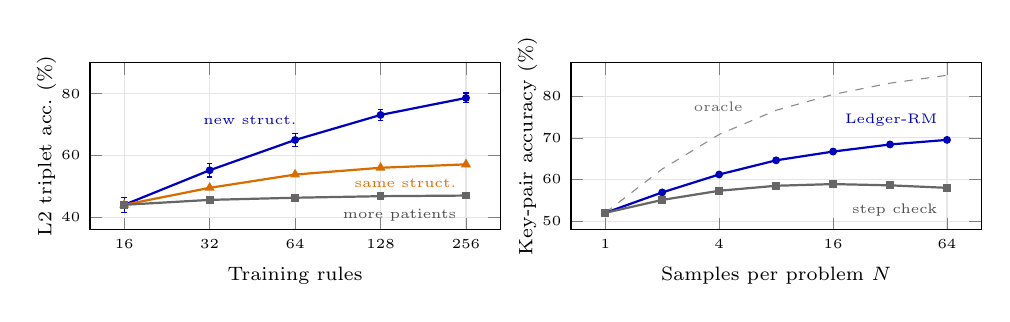
\begin{tikzpicture}
\begin{axis}[name=div, width=0.56\linewidth, height=3.7cm,
  xmode=log, log basis x=2, xtick={16,32,64,128,256},
  xticklabels={16,32,64,128,256},
  xlabel={Training rules}, ylabel={L2 triplet acc.\ (\%)},
  ymin=36, ymax=90,
  tick label style={font=\tiny}, label style={font=\scriptsize},
  ylabel style={yshift=-5pt}, grid=major, grid style={black!10}]
\addplot[blue!75!black, thick, mark=*, mark size=1pt, error bars/.cd, y dir=both, y explicit]
  coordinates {(16,44.0) +- (0,2.4) (32,55.2) +- (0,2.2) (64,65.0) +- (0,2.0) (128,73.1) +- (0,1.8) (256,78.6) +- (0,1.6)};
\addplot[orange!85!black, thick, mark=triangle*, mark size=1.3pt]
  coordinates {(16,44.0)(32,49.5)(64,53.8)(128,56.0)(256,57.1)};
\addplot[black!60, thick, mark=square*, mark size=1pt]
  coordinates {(16,44.0)(32,45.6)(64,46.3)(128,46.8)(256,47.0)};
\node[font=\tiny, blue!75!black, anchor=south east] at (axis cs:70,67) {new struct.};
\node[font=\tiny, orange!85!black, anchor=north east] at (axis cs:256,55.6) {same struct.};
\node[font=\tiny, black!70, anchor=north east] at (axis cs:256,45.8) {more patients};
\ifplaceholders\node[red, font=\tiny\bfseries, opacity=0.5] at (rel axis cs:0.33,0.92) {PLACEHOLDER};\fi
\end{axis}
\begin{axis}[at={(div.east)}, anchor=west, xshift=9mm,
  width=0.56\linewidth, height=3.7cm,
  xmode=log, log basis x=2, xtick={1,4,16,64}, xticklabels={1,4,16,64},
  xlabel={Samples per problem $N$}, ylabel={Key-pair accuracy (\%)},
  ymin=48, ymax=88,
  tick label style={font=\tiny}, label style={font=\scriptsize},
  ylabel style={yshift=-5pt}, grid=major, grid style={black!10}]
\addplot[blue!75!black, thick, mark=*, mark size=1pt]
  coordinates {(1,52.0)(2,56.9)(4,61.2)(8,64.6)(16,66.7)(32,68.4)(64,69.5)};
\addplot[black!60, thick, mark=square*, mark size=1pt]
  coordinates {(1,52.0)(2,55.1)(4,57.3)(8,58.5)(16,58.9)(32,58.6)(64,58.0)};
\addplot[black!45, dashed]
  coordinates {(1,52.0)(2,62.5)(4,70.8)(8,76.6)(16,80.4)(32,83.1)(64,85.0)};
\node[font=\tiny, blue!75!black, anchor=south east] at (axis cs:64,70.5) {\method};
\node[font=\tiny, black!70, anchor=north east] at (axis cs:64,56.5) {step check};
\node[font=\tiny, black!60, anchor=south east] at (axis cs:6,74) {oracle};
\ifplaceholders\node[red, font=\tiny\bfseries, opacity=0.5] at (rel axis cs:0.33,0.93) {PLACEHOLDER};\fi
\end{axis}
\end{tikzpicture}
\caption{Left: L2 triplet accuracy of \method{} as training grows by adding
rules of new structures, rules of structures already seen, or only patients for
\ph{16} fixed rules (same data size; bars: s.d.\ over seeds). Right: accuracy
on both members of a MedQA key pair for the trace selected among $N$ samples.}
\label{fig:diversity}
\end{figure}

\emph{A decision bit explains most of the rule-tier gain.} If the reader also
writes whether the condition applies, a judge that sees only that bit and the
claim reaches \ph{77.5}\% on L2, against \ph{78.6}\% for the fact-only ledger.
On rules the benefit therefore lies in what the reader is trained to
establish, not in the judge's use of the fields. The fields matter in
transfer: \ph{38.2}\% against \ph{44.8}\% on MedEinst zero-shot
(Table~\ref{tab:ablation}). They also matter as supervision: a reader trained
to write the bit without fields reaches \ph{63.0}\%.

\emph{The reader is the bottleneck.} With program-supplied ledgers the judge
solves \ph{96.5}\% of L2 triplets, so about \ph{84}\% of the errors of the
full model arise in the reader. A second pass that re-reads each entry against
the case and regenerates rejected ones raises triplet accuracy to
\ph{81.3}\%.

\emph{Direct access to the case trades selectivity for coverage.} A one-stage
variant, in which the ledger is written as a rationale and the verdict is
produced with the case in context, solves \ph{71.6}\% of L2 triplets, holds on
\ph{80.2}\% of near-misses against \ph{86.9}\%, and is \ph{2.7} points better
on MedEinst zero-shot. Where a few typed fields cannot carry the evidence, the
bottleneck costs accuracy.

\emph{Field interventions.} Changing \texttt{subject}, \texttt{status} or
\texttt{time} in a correct ledger changes the verdict as the program
prescribes in \ph{97.3}\% of cases, and given the ledger of another case the
judge returns the verdict that ledger implies in \ph{96.8}\%
(Appendix~\ref{app:ledger}). Figure~\ref{fig:diversity} (left): rules of new
signature classes raise L2 accuracy from \ph{44.0}\% to \ph{78.6}\%, rules of
seen classes to \ph{57.1}\%, more patients to \ph{47.0}\%.

\subsection{Candidate selection}
\label{sec:results-downstream}

\begin{table}[t]
\centering\small
\setlength{\tabcolsep}{2.4pt}
\begin{tabular}{@{}lcccccc@{}}
\toprule
 & \multicolumn{2}{c}{Accuracy} & Key & \multicolumn{3}{c}{MedEinst}\\
\cmidrule(lr){2-3}\cmidrule(lr){5-7}
Selection & MQA & CQA & pair & pair & ctrl & trap\\
\midrule
Single sample          & \ph{71.2} & \ph{66.8} & \ph{52.0} & \ph{31.2} & \ph{78.5} & \ph{39.8}\\
Self-consistency       & \ph{74.5} & \ph{70.1} & \ph{55.8} & \ph{33.5} & \ph{81.0} & \ph{41.4}\\
Step check             & \ph{77.6} & \ph{72.4} & \ph{58.9} & \ph{34.0} & \ph{81.2} & \ph{41.9}\\
\ \ \ vignette swapped & \ph{76.8} & \ph{71.9} & \ph{57.6} & \ph{33.6} & \ph{80.9} & \ph{41.5}\\
Ledger score           & \ph{76.0} & \ph{71.0} & \ph{65.1} & \ph{44.7} & \ph{81.3} & \ph{54.9}\\
Combined               & \ph{78.3} & \ph{73.0} & \ph{66.7} & \ph{45.9} & \textbf{\ph{82.0}} & \ph{55.6}\\
\ \ \ vignette swapped & \ph{73.9} & \ph{69.2} & \ph{54.1} & \ph{32.8} & \ph{80.1} & \ph{40.6}\\
\ \ \ no near-misses   & \ph{77.1} & \ph{72.2} & \ph{64.9} & \textbf{\ph{46.5}} & \ph{81.0} & \textbf{\ph{56.8}}\\
\ph{Claude Opus 5.5}   & \textbf{\ph{79.5}} & \textbf{\ph{76.0}} & \textbf{\ph{70.2}} & \ph{44.1} & \textbf{\ph{82.0}} & \ph{53.8}\\
\midrule
Oracle selection       & \ph{88.0} & \ph{85.3} & \ph{80.4} & \ph{58.7} & \ph{90.2} & \ph{65.1}\\
\bottomrule
\end{tabular}
\caption{Reranking \ph{16} samples of a \bb{} policy on identical pools (\%).
MQA: MedQA; CQA: CareQA. Step check: injected-error PRM. Ledger score:
\method{} trained on rule triplets and clinical pairs. Combined: minimum of
the two after calibration.}
\label{tab:downstream}
\end{table}

Table~\ref{tab:downstream} tests selection among samples of a fixed policy.
The combined reward and the step check improve accuracy on MedQA and CareQA
by similar amounts (difference \ph{0.7} [\ph{$-$0.2}, \ph{1.6}] on MedQA,
non-inferior at a margin of one point). On both members of a key pair the
combined reward reaches \ph{66.7}\% against \ph{58.9}\%, and on MedEinst pairs
\ph{45.9}\% against \ph{34.0}\%, with control accuracy unchanged. Swapping in
the vignette of another question removes the gain of the combined reward and
leaves the step check almost unchanged: the ledger score depends on the
supplied case. That the dependence is correct is what the pair columns show.
Without near-misses in training the combined reward loses \ph{1.2} points on
MedQA and nothing on MedEinst, whose pairs contain no near-misses. As $N$
grows, pair accuracy under the step check stays flat while the oracle rises
(Figure~\ref{fig:diversity}, right).

\section{Conclusion}

On executable rules, reward models fail in two directions. The remedy has two
parts: balanced training with near-misses, and a record of what the case says,
whose it is and when, from which a case-blind judge decides. Trained on
rules alone, this carries to rules of unseen structure and, in part, to
existing clinical pair labels. Holding on inapplicable evidence in clinical
text is not established.

\section*{Limitations}

\textbf{What the labels are.} Rule-tier labels are exact relative to a stated
rule, its applicability predicates and a rendering grammar. They say what the
rule implies, not what is clinically optimal. We commissioned no new clinical
annotation; reused benchmarks carry the review their authors report.
Clinical-tier results are agreement with released labels: MedEinst cases
derive from a simulator and were edited and filtered by the benchmark, key
pairs inherit the errors of exam keys and are not counterfactuals, NLI4CT-P
edits statements about breast-cancer trial reports. Nothing here supports
clinical use.

\textbf{Selectivity outside rules is tested only indirectly.} Applicability near-misses
with exact labels require a rule program. On the clinical tier, holding is tested only on
the claim side: by NLI4CT-P consistency under statement edits and by
expert-reviewed distractors in real discharge summaries that attribute a
correct fact to the wrong admission \citep{kim2026ehrnotechatqa}
(Appendix~\ref{app:qa}). No existing benchmark edits the case in this way;
assertion annotations of clinical notes \citep{uzuner2011i2b2} would allow a
test of the reader alone.

\textbf{The bottleneck.} The ledger assumes that a claim depends on a few
identifiable findings with a subject, status and time. Claims that weigh many
soft findings fit it poorly, and the one-stage variant is better on MedEinst.
The judge computes its verdict from the ledger; nothing guarantees that the
ledger is right, and a quotation can exist in the case and still be the wrong
evidence.

\textbf{Rule population.} Rules come from one calculator benchmark, our
implementations of published scores, stated constraints and a grammar;
templates are cleaner than clinical notes. Held-out signature classes share
operators with training rules.

\textbf{Weak supervision.} For rows trained on clinical pairs, ledger targets
come from differences between paired cases and from selection with a frozen
judge; they are not verified.

\textbf{Interpretation and scope.} The composition gap and shift classes are
descriptive. Reranking tests selection for one policy. All data are in
English.

\section*{Ethical Considerations}

The work uses public benchmarks and synthetic patients; no patient data were
collected. Stated rules in our data are test specifications and must not be
read as prescribing guidance. A reward model that appears to check patient
evidence could be trusted more than it should be; accuracy on these triplets
does not establish safety in care, and the models are released for research on
post-training only. Because the engine generates cases on which a given reward
fails, it could be used to construct inputs that mislead a deployed evaluator;
we see this as an argument for auditing rewards before they are used.

\bibliography{custom}

\appendix

\section{Analysis Plan}
\label{app:plan}

\ifplaceholders
\noindent\textcolor{red}{\textbf{Draft status.} No experiment in this
manuscript has been run. Every value printed in red, and every curve marked as
placeholder data, is a target value used to lay out the paper. This paragraph
and the red banner disappear, and the build fails on any remaining
placeholder, once measured values are entered.}\smallskip
\fi

\noindent\textbf{Primary endpoints.} Triplet accuracy on L2 (rendered text,
rule stated) and reversal on MedEinst test pairs for the model trained on
rule triplets only.

\noindent\textbf{Primary comparisons} (paired, Holm-corrected): on L2,
(1) balanced against natural, verdict only; (2) triplets against blocks,
verdict only; (3) applicability ledger against two-stage evidence summary,
triplets; on MedEinst, (4) rule-only \method{} against the untrained critic;
(5) rule-only \method{} against the rule-only evidence summary.

\noindent\textbf{Decision rules.} If (2) fails, near-misses are reported as an
evaluation device only. If (3) fails, the paper is a data-design result. If
(4) fails, the answer outside rules is negative. If the gain in (4) appears
only with step-error data, it is reported as a gain from medical supervision.

\noindent\textbf{Selection and freezing.} Hyperparameters, thresholds, the
calibration of the combined reward and the choice of headline system use
development splits only: development triplets from training-fold signature
classes and a held-out part of the MedEinst reference set. Test sets are
generated or opened after these choices are frozen and are evaluated once.

\section{Rule Library and Splits}
\label{app:rules}

\begin{table}[!ht]
\centering\small
\setlength{\tabcolsep}{4pt}
\begin{tabular}{@{}lrr@{}}
\toprule
Source & Rules & Classes\\
\midrule
MedCalc-Bench calculators (audited) & \ph{48}  & \ph{9}\\
Published scores, our implementation & \ph{90} & \ph{11}\\
Stated constraint rules             & \ph{120} & \ph{5}\\
Grammar-sampled rules               & \ph{300} & \ph{19}\\
\bottomrule
\end{tabular}
\caption{Rule population. Classes overlap across sources; \ph{19} in total.}
\label{tab:rules}
\end{table}

\paragraph{Sources.}
We use the calculator programs released with MedCalc-Bench. Further scores
are implemented from their published definitions; the manifest gives the
source of each, the rule text shown in prompts, the program and its tests. We
do not use the calculator set of MedCalc-Eval \citep{mao2025medcalceval},
whose definitions were not available to us. Because every prompt states the
rule, correctness is relative to the stated text for all four sources.

\paragraph{Constraint rules and claims.}
Each rule states a default option, a condition and an alternative. It is
derived from a public drug-label or guideline recommendation in three steps
taken from \citet{shen2026medguidex}, whose own functions are not released: a
model extracts the recommendation, writes it as a decision tree, and compiles
the tree to a program. We keep a rule if the tree is complete, the program
passes the boundary tests and agrees with the tree on sampled inputs, and
show the verbalised tree in the prompt. No clinician checks the tree against
the source, which is why labels are relative to the stated rule. Options
are plain orders of one form (drug, dose, route, frequency, duration) that
differ by at most \ph{2} tokens and contain no word that gives a reason.
Every case reports the same fields with raw values, so the presence of a
field carries no label information. Swapping which option is the default, or
paraphrasing the options, changes triplet accuracy of \method{} by at most
\ph{0.9} points.

\paragraph{Splits and overlap.}
In each of \ph{3} folds \ph{5} of \ph{19} signature classes are held out for
L2. Between training and L2 rules, \ph{0}\% of canonical programs,
\ph{12.4}\% of criterion subexpressions, \ph{0}\% of rule texts and \ph{0}\%
of rendering templates and cue phrases are shared: each input type has
\ph{6} templates, \ph{4} for training and \ph{2} for test, and the words
that mark relatives, negation and time are split in the same way. With
training templates and cues on the same L2 rules, triplet accuracy is
\ph{81.4}\% for \method{}, against \ph{78.6}\% with held-out ones. L3-alt
moves one or two thresholds and keeps only cases whose outcome differs between
the original and the altered rule.

\section{Triplet Construction}
\label{app:twins}

\paragraph{Invariants.}
Of the proposed flips, \ph{7.9}\% are discarded because a second criterion
changes; of the proposed missing twins, \ph{18.6}\% because the remaining
inputs determine the criterion. Near-misses are checked by executing the
program on the state recovered from the rendered case, and the equalities
$h_k(x)=0$, $h_k(\xf)=h_k(\xn)=1$ (or $h_k\equiv 1$ for measured inputs) are
checked on the rendered text of every triplet. Per fold the training
set has \ph{16{,}000} triplets over \ph{370} rules and L2 has \ph{8{,}000}
over \ph{130}. The authors inspected \ph{300} rendered triplets, stratified by
edit kind, for rendering errors and found \ph{2}; this checks the grammar and
not clinical validity.

\paragraph{Near-miss kinds.}
Numeric \ph{40}\%, other subject \ph{20}\%, absent status \ph{20}\%, time
outside the predicate \ph{20}\%. For criteria whose predicate counts past or
family findings, such mentions are flips.

\paragraph{Text tiers.}
Notes rewritten by \ph{Gemma-3-27B} are accepted if two extractors recover
the intended state (\ph{8.7}\% rejected). \method{} reaches \ph{74.8}\% on
accepted and \ph{60.3}\% on rejected groups relabelled from the intended
state, so the filter removes harder text.

\section{Clinical Tier}
\label{app:qa}

\paragraph{Releases.}
MedEinst as released by its authors; NLI4CT-P as distributed for SemEval-2024
Task~2; MedPRMBench and CareQA at pinned revisions listed in the repository.

\paragraph{MedEinst.}
Claims are the two diagnoses. For training rows, the \texttt{found} targets
are the findings in which the two cases differ, taken from the structured
evidence where released and from a token diff otherwise; the two agree on
\ph{96.2}\% of a sample of \ph{500} pairs, and in \ph{97} of \ph{100} pairs
inspected by the authors the difference names the edited finding. Other ledger fields are not
supervised there. In the disease-held-out split a pair is in the test set
only if both of its diagnoses are test diseases (\ph{12} of 49), and in the
training set only if both are training diseases.

\paragraph{Key pairs.}
Pairs are mined within a split and reduced to a one-to-one matching, so that
no question occurs in two pairs. Excluded: negatively phrased lead-ins,
options that refer to other options, and questions without a case
description. For training rows, ledgers are sampled once from the frozen
rule-trained reader and kept if their quotations occur in the case and the
frozen rule-trained judge returns the keyed verdict on all four cells
(\ph{38.5}\% kept); the kept set is fixed and shared by all ledger formats. By
tercile of vignette similarity, reversal of the critic is \ph{55.7}\%,
\ph{44.1}\% and \ph{33.8}\%. CareQA covers six subject areas; results by area
are in the repository, and the biology and chemistry areas contribute
\ph{4}\% of pairs.

\paragraph{CondMedQA.}
CondMedQA \citep{parekh2026cgr} has 100 questions that contain a patient
condition, each with the answer given the condition and the general answer
that would hold without it; candidates were generated by a model, verified by
its authors, and 30 were reviewed by annotators with medical expertise. We
score both answers as claims for the question as posed and count how often
the condition-specific answer is preferred: \ph{41.0}\% for the critic,
\ph{56.0}\% for rule-only \method{} [\ph{46}, \ph{66}] and \ph{80.0}\% for the
closed judge. This is a test of resisting the default answer and not a
reversal pair, since the benchmark has no version of the question without the
condition; no rule is stated, so it also measures knowledge.

\paragraph{Claim-side applicability on real notes.}
EHRNote-ChatQA \citep{kim2026ehrnotechatqa} asks questions about a patient's
discharge summaries, each with one correct and four incorrect answers that
follow defined patterns and were reviewed by medical experts. Two patterns
mirror our near-misses on the claim side: a correct fact attributed to the
wrong admission, and a related entity or attribute taken from elsewhere in the
notes. Scoring each answer as a claim against the notes, the correct answer is
preferred to such a distractor in \ph{58.0}\% of cases by the critic, in
\ph{69.5}\% by rule-only \method{} and in \ph{77.0}\% with clinical pairs.
The data are under credentialed access and may not be sent to external
services, so closed judges are not evaluated on them.

\paragraph{NLI4CT-P.}
Base macro-F1 is \ph{71.0} for the critic and \ph{76.4} for rule-only
\method{}; joint correctness over an original statement and all its
interventions is \ph{38.5}\% and \ph{47.9}\%. Faithfulness and consistency follow the task definitions; pairs
that share an original statement are resampled together.

\paragraph{Overlap.}
By normalised question text, CareQA shares no question with MedQA. The MedQA
portion of ReMedQA \citep{cocchieri2026remedqa} lies within the MedQA test
split; we do not use ReMedQA.

\section{Ledger Format and Scoring}
\label{app:ledger}

{\footnotesize
\begin{verbatim}
need: penicillin allergy in the patient
found: "penicillin allergy (anaphylaxis)"
subject: other (mother)
status: present
time: current
\end{verbatim}}

\noindent Given this ledger, the rule and the claim ``Order amoxicillin'', the
judge returns \texttt{+}. Malformed ledgers occur in \ph{0.4}\% of rule-tier
and \ph{2.4}\% of MedEinst instances. Temperature scaling for the combined
reward is fitted on development data separately for the two scores. The
verification pass prompts the same adapter with one ledger entry and the case
and asks whether value, subject, status and time are as recorded; it rejects
\ph{41}\% of wrong entries and \ph{3.2}\% of correct ones. In
triplet and pair evaluations one ledger serves both claims. In selection the
reader receives a step; for two candidate steps about the same criterion the
ledgers are identical in \ph{98.7}\% of cases. On L2 the reader is right on \ph{96.9}\%, \ph{95.4}\% and \ph{94.1}\% of
\texttt{found}, \texttt{subject} and \texttt{time} fields. In \ph{2.1}\% of
L2 cases it quotes a span that occurs in the case and is not the decisive
finding;
the string check cannot detect this.

\section{Diagnostics}
\label{app:diag}

\begin{table}[!ht]
\centering\small
\setlength{\tabcolsep}{4pt}
\begin{tabular}{@{}lccc@{}}
\toprule
Scorer (L2) & Rev & Hold & TA\\
\midrule
Always default                 & 0 & 100 & 0\\
Claim only                     & 0 & --  & 0\\
Concept named ($h_k$)          & $\le$\,\ph{45} & -- & 0\\
Attribute-blind, logistic      & \ph{85.0} & \ph{41.0} & \ph{27.2}\\
\ \ applicability triplets     & \ph{93.0} & \ph{11.5} & \ph{6.3}\\
Bag of words, case + claim     & \ph{31.0} & \ph{55.0} & \ph{9.2}\\
Trigger lexicon + program      & \ph{88.0} & \ph{58.5} & \ph{52.0}\\
\ \ with training cue phrases  & \ph{97.0} & \ph{93.5} & \ph{91.0}\\
\bottomrule
\end{tabular}
\caption{Shortcut scorers (\%). Uncoloured entries follow from
Proposition~\ref{prop:blind}. Concept named: any deterministic scorer that
uses the case only through $h_k$; in \ph{45}\% of triplets the flip
introduces the decisive finding. Attribute-blind: a logistic model on
concept--value features without subject, status and time. Trigger lexicon: a
rule-based reader with negation, experiencer and temporality triggers in the
style of ConText \citep{harkema2009context}, built from training cue phrases,
followed by the rule program; its drop on held-out cue phrases is why test
cues are held out.}
\label{tab:shortcuts}
\end{table}

\begin{table}[!ht]
\centering\small
\setlength{\tabcolsep}{3.2pt}
\begin{tabular}{@{}lcccccc@{}}
\toprule
Signal & Base & Ties & UR ($n$) & $P$ & $K$ & $G$\\
\midrule
Inj.-error PRM       & \ph{93.5} & \ph{0.0} & \ph{8.1} (\ph{4{,}769})  & \ph{92.8} & \ph{89.5} & \ph{71.4}\\
Qwen3-8B             & \ph{80.2} & \ph{0.0} & \ph{24.6} (\ph{4{,}090}) & \ph{95.3} & \ph{91.2} & \ph{56.8}\\
Qwen3-32B            & \ph{88.4} & \ph{0.0} & \ph{26.0} (\ph{4{,}508}) & \ph{97.6} & \ph{95.4} & \ph{33.4}\\
\ph{Claude Opus 5.5} & \ph{96.0} & \ph{3.8} & \ph{12.9} (\ph{4{,}896}) & \ph{99.2} & \ph{98.1} & \ph{11.3}\\
\bottomrule
\end{tabular}
\caption{L0 (\%). Base accuracy; tied preferences; unnecessary reversal among
triplets with a correct base preference, with its denominator; reading and
application reversal; composition gap.}
\label{tab:pk}
\end{table}

\paragraph{Shift relative to a missing-input baseline.}
Let $d_0=d(\xm)$, $\delta(x)=d(x)-d_0$, and $y\in\{+1,-1\}$ the correct sign
of $d(x)$. For cases with $y\,d_0<0$, where the baseline preference opposes
the label, $y\,d(x)=-|d_0|+y\,\delta(x)$, so the preference is right if and
only if
\begin{equation}
y\,\delta(x) > |d_0| .
\label{eq:margin}
\end{equation}
Cases with $d_0=0$ have no opposing baseline and are counted separately. We
sort the others into four disjoint classes, in this order: \emph{crossed}
(Eq.~\ref{eq:margin}); \emph{unmoved} ($|\delta|\le\tau$, the model's median
$|d(x^{\mathrm{p}})-d(x)|$ over presentation edits); \emph{wrong direction}
($y\delta<0$); \emph{short}. The split restates the decision rule and adds the
direction and relative size of the shift. The \emph{shift ratio} compares that
size with the model's response to an error inside a step:
\begin{equation}
\kappa=\frac{\operatorname{med}\{\,y\,\delta(x): y\,d_0<0\,\}}
{\operatorname{med}\{\,u(s^{+},x)-u(s^{-},x)\,\}},
\label{eq:kappa}
\end{equation}
where the denominator runs over matched pairs of a correct step $s^{+}$ and
its injected-error version $s^{-}$ on the same case in the MedPRMBench
development split; both medians are in log-odds, and $\kappa$ is reported
with a bootstrap interval when the denominator is positive.
For the injected-error PRM, \ph{16.8}\% of baseline-conflicting cases cross,
\ph{55.2}\% move the right way and fall short, \ph{19.5}\% do not move and
\ph{8.5}\% move the wrong way; $\kappa=\ph{0.18}$
(Figure~\ref{fig:diagnosis}).

\begin{figure}[!ht]
\centering
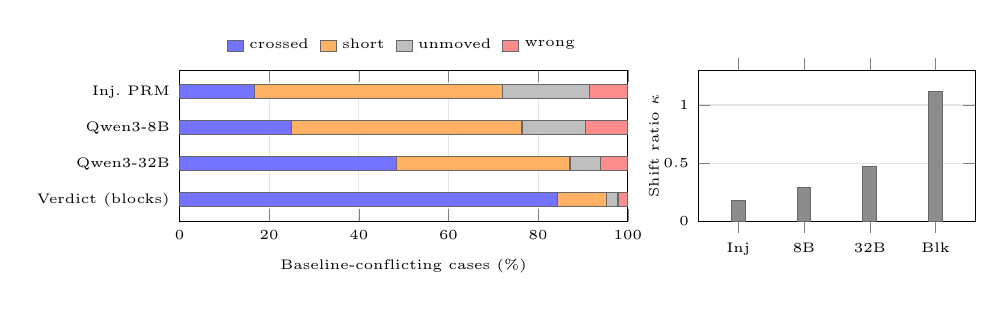
\begin{tikzpicture}
\begin{axis}[name=tax, xbar stacked, width=0.60\columnwidth, height=3.5cm,
  xmin=0, xmax=100, bar width=5pt,
  ytick={1,2,3,4}, yticklabels={Verdict (blocks),Qwen3-32B,Qwen3-8B,Inj.\ PRM},
  ymin=0.4, ymax=4.6,
  tick label style={font=\tiny}, label style={font=\tiny},
  xlabel={Baseline-conflicting cases (\%)},
  legend style={font=\tiny, at={(0.5,1.04)}, anchor=south, legend columns=4,
                draw=none, /tikz/every even column/.append style={column sep=2pt}},
  legend image code/.code={\draw[#1] (0cm,-0.07cm) rectangle (0.2cm,0.07cm);},
  ymajorgrids=false, xmajorgrids, grid style={black!10}]
\addplot[fill=blue!55,   draw=black!60] coordinates {(84.3,1) (48.5,2) (25.0,3) (16.8,4)};
\addplot[fill=orange!60, draw=black!60] coordinates {(11.0,1) (38.6,2) (51.4,3) (55.2,4)};
\addplot[fill=black!25,  draw=black!60] coordinates {(2.5,1)  (6.9,2)  (14.1,3) (19.5,4)};
\addplot[fill=red!45,    draw=black!60] coordinates {(2.2,1)  (6.0,2)  (9.5,3)  (8.5,4)};
\legend{crossed,short,unmoved,wrong}
\phmark{rel axis cs:0.5,0.5}
\end{axis}
\begin{axis}[at={(tax.east)}, anchor=west, xshift=9mm, ybar,
  width=0.42\columnwidth, height=3.5cm, bar width=5pt,
  ymin=0, ymax=1.3, ytick={0,0.5,1},
  symbolic x coords={Inj,8B,32B,Blk}, xtick=data,
  tick label style={font=\tiny}, label style={font=\tiny},
  ylabel={Shift ratio $\kappa$}, ylabel style={yshift=-5pt},
  enlarge x limits=0.2, ymajorgrids, grid style={black!10}]
\addplot[fill=black!45, draw=black!60] coordinates {(Inj,0.18) (8B,0.29) (32B,0.47) (Blk,1.12)};
\phmark{rel axis cs:0.5,0.82}
\end{axis}
\end{tikzpicture}
\caption{Rule tier. Left: cases whose correct preference opposes the
missing-input baseline, by class (Eq.~\ref{eq:margin}; models that expose
log-probabilities). Right: shift ratio $\kappa$ (Eq.~\ref{eq:kappa}). Verdict
(blocks): the verdict-only model trained on flip blocks.}
\label{fig:diagnosis}
\end{figure}

\paragraph{Readouts and sampling noise.}
Dedicated PRMs use their released scoring head, open judges the log-odds of
the verdict token, and API judges without log-probabilities the verdict
frequency over \ph{32} samples at temperature \ph{1.0}, for which the standard
error of a frequency is at most \ph{0.09}. Scoring Qwen3-32B by the same
sampling protocol lowers its triplet accuracy from \ph{45.3}\% to
\ph{42.0}\%, with \ph{4.1}\% ties.

\paragraph{Input ablations.}
Replacing the question stem by ``No case description is available'' lowers
PRMScore on MedPRMBench by \ph{1.2}--\ph{2.9} points for trained PRMs. This is
an input ablation and not a measure of grounding: many injected errors are
detectable within the step, and chains restate patient facts. On the error
types that the benchmark defines relative to the case the loss is
\ph{4.0}--\ph{9.5} points, and \ph{6.2}--\ph{13.0} when numbers and quoted
spans of the stem are also masked in the chain.

\paragraph{Exploratory.}
A probe on the residual stream of the critic predicts the criterion outcome on
held-out signature classes with \ph{90.8}\% accuracy (control task
\citep{hewitt2019control}: \ph{49.6}\%); decodability does not show use
\citep{elazar2021amnesic}.

\section{Additional Results}
\label{app:more}

\begin{table}[!ht]
\centering\small
\setlength{\tabcolsep}{3pt}
\begin{tabular}{@{}lccccc@{}}
\toprule
Variant (rule triplets only) & Rev & Hold & TA & MR & ME\\
\midrule
\method{} (facts only)        & \ph{91.0} & \ph{86.9} & \ph{78.6} & \ph{84.6} & \ph{44.8}\\
\ \ + decision field          & \ph{91.3} & \ph{87.4} & \ph{79.2} & \ph{84.9} & \ph{44.1}\\
\ \ decision field only       & \ph{90.8} & \ph{86.0} & \ph{77.5} & \ph{83.0} & \ph{38.2}\\
\ \ program on predicted bit  & \ph{90.9} & \ph{86.2} & \ph{77.8} & \ph{83.1} & --\\
\ \ reader writes bit only    & \ph{80.5} & \ph{74.0} & \ph{63.0} & \ph{79.0} & \ph{34.5}\\
\ \ + verification pass       & \ph{92.0} & \ph{89.1} & \ph{81.3} & \ph{85.6} & \ph{45.4}\\
\ \ program-supplied ledger   & \ph{98.6} & \ph{97.8} & \ph{96.5} & \ph{97.0} & --\\
One-stage ledger              & \ph{88.1} & \ph{80.2} & \ph{71.6} & \ph{82.3} & \ph{47.5}\\
Value ledger                  & \ph{90.4} & \ph{76.4} & \ph{68.3} & \ph{83.5} & \ph{42.0}\\
Evidence summary              & \ph{89.0} & \ph{74.8} & \ph{66.5} & \ph{80.4} & \ph{39.4}\\
Concept scorer                & \ph{84.5} & \ph{78.0} & \ph{65.9} & \ph{76.2} & \ph{31.0}\\
Premise gate                  & \ph{62.0} & \ph{79.5} & \ph{49.3} & \ph{70.1} & \ph{30.5}\\
$-$ near-misses               & \ph{90.2} & \ph{49.0} & \ph{44.0} & \ph{83.9} & \ph{46.3}\\
\ \ + probe re-weighting       & \ph{84.0} & \ph{60.5} & \ph{50.8} & \ph{83.0} & \ph{44.0}\\
$-$ presentation edits        & \ph{90.6} & \ph{82.0} & \ph{73.5} & \ph{84.2} & \ph{44.5}\\
$-$ ledger resampling         & \ph{89.7} & \ph{85.5} & \ph{76.9} & \ph{84.0} & \ph{44.0}\\
Verdict only, pairwise loss   & \ph{77.0} & \ph{71.2} & \ph{53.6} & \ph{60.5} & \ph{33.8}\\
\bottomrule
\end{tabular}
\caption{Ablations on L2 and MedEinst zero-shot (\%). Decision field: the
reader also writes whether the condition applies. Verification pass: every
entry is re-read against the case and regenerated once if rejected, after
\citet{agand2026venra}. Program-supplied ledger: the judge receives the target
ledger. Concept scorer: fields
predicted by linear heads and a linear verdict. Premise gate: the step check,
attenuated toward a neutral score when the finding a step relies on is not
supported by a ledger extracted once per case, after \citet{evpv2026}. Probe
re-weighting: near-misses are not trained on; base--flip pairs whose
preference shifts under near-miss and presentation edits are down-weighted,
after \citet{liu2026dynacf}. Pairwise loss: Bradley--Terry on the two claims.}
\label{tab:ablation}
\end{table}

\begin{table}[!ht]
\centering\small
\setlength{\tabcolsep}{3.2pt}
\begin{tabular}{@{}lcccc@{}}
\toprule
System & L0 & L1 & L2 & FR\\
\midrule
Critic                   & \ph{27.9} & \ph{26.3} & \ph{25.1} & \ph{5.3}\\
Verdict only, triplets   & \ph{79.3} & \ph{64.0} & \ph{52.4} & \ph{5.6}\\
\method{}, rule triplets & \ph{92.4} & \ph{85.5} & \ph{78.6} & \ph{5.2}\\
Closed judge, ledger     & \ph{86.7} & \ph{85.9} & \ph{85.1} & \ph{5.4}\\
\bottomrule
\end{tabular}
\caption{Rule ladder (triplet accuracy, \%) and achieved false rejection on
L2 at the development threshold. Rejection curves over thresholds and
per-class results are in the repository;
the lowest held-out class is at \ph{66.0}\% for \method{}.}
\label{tab:ladder}
\end{table}

\paragraph{Training.}
LoRA rank \ph{64}, learning rate \ph{1e-4}, batch size \ph{64}, \ph{2} epochs,
$\lambda=\ph{1.0}$, $p=\ph{0.3}$. Rows with clinical pairs mix rule triplets
and pairs \ph{1}:\ph{1}.

\paragraph{Resources.}
Per scored claim: verdict only, \ph{1} pass and \ph{1} generated token;
\method{}, \ph{2} passes and \ph{45} tokens; generated-program verifier,
\ph{1} pass, \ph{540} tokens and one execution; GenPRM-style verifier,
\ph{1} pass, \ph{500} tokens and one execution; closed judge with ledger
prompt, \ph{1} API call and \ph{210} tokens, about \ph{60} times the list
price of the 8B model per claim. Latency and hardware are in the repository.

\paragraph{Policy training.}
GRPO from one \bb{} initialisation on rule triplets, \ph{3} runs, \ph{8}
rollouts per prompt, \ph{2000} steps, advantages standardised within a group.
Before each run we check that reward terms are not collinear within groups
and that the setup fits a \ph{64}-prompt subset. Accuracy on base--flip pairs
of held-out structures, judged by the rule program, moves from \ph{38.6}\% to
\ph{52.3}\% with an outcome reward, \ph{33.9}\% with the injected-error PRM
and \ph{63.5}\% with \method{}. A reference-graph reward after
\citet{medceg2025}, which scores a rollout by its coverage of the decisive
findings and of the chain from finding to criterion to conclusion, gives
\ph{58.0}\%; the rule program supplies the graph, so this reward, like the
outcome reward, uses the answer for each case.

\paragraph{Selection protocol.}
A trace is eligible if it contains a final answer (\ph{6.1}\% are not).
Ranking by the product of the two calibrated scores gives \ph{78.0}\% on
MedQA and \ph{66.1}\% on key pairs, a logistic combination fitted on
development data \ph{78.5}\% and \ph{67.0}\%, and the minimum \ph{78.3}\% and
\ph{66.7}\%. With
a paraphrased vignette the combined reward gives \ph{78.0}\% on MedQA. For
nested pools the selected reward cannot fall as $N$ grows, so we report
selection regret, the gap between oracle and selected accuracy: at $N=64$ it
is \ph{27.0} points for the step check and \ph{15.5} for the combined reward
on key pairs. On the open-ended version of CareQA, graded against reference
answers by a fixed model grader, the share graded correct moves from
\ph{48.2}\% to \ph{51.0}\%; this check is exploratory.

\ifplaceholders\else
\section{Reproducibility}
\label{app:repro}
Every number in this paper is produced by a script that writes the
corresponding table or figure. The rule manifest, the grammar, the triplet
engine, the key-pair miner, prompts, splits, model revisions and trained
adapters are released with the paper.
\fi

\end{document}
